\documentclass[11pt, oneside]{article}   	% use "amsart" instead of "article" for AMSLaTeX format
\usepackage{geometry}                		% See geometry.pdf to learn the layout options. There are lots.
\geometry{letterpaper}                   		% ... or a4paper or a5paper or ... 
%\geometry{landscape}                		% Activate for rotated page geometry
%\usepackage[parfill]{parskip}    		% Activate to begin paragraphs with an empty line rather than an indent
\usepackage{graphicx,wrapfig}				% Use pdf, png, jpg, or eps§ with pdflatex; use eps in DVI mode
								% TeX will automatically convert eps --> pdf in pdflatex		
\usepackage{amssymb}

%SetFonts

%SetFonts


\title{Brief Article}
\author{The Author}
%\date{}							% Activate to display a given date or no date

\begin{document}
%\maketitle
%\section{}
%\subsection{}
\hfill Donovan Guelde

\hfill CSCI 5622

\hfill Boosting HW\\

Using Sklearn's Adaboost with the DecisionTreeClassifier, the dataset was analyzed, and the accuracy of distinguishing 4's from 9's was established.  At a tree depth of 1, 2, and 3, with n\_learners=100, 200, 300, 400, 500, and 1000 for each tree depth, the following results were obtained:\\
\begin{wrapfigure}{r}{8cm}
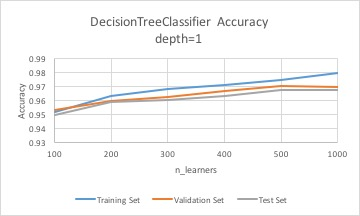
\includegraphics[width=8cm]{decisionTree1} 
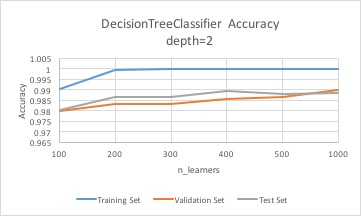
\includegraphics[width=8cm]{decisionTree2} 
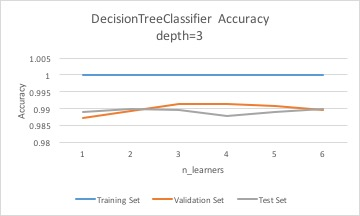
\includegraphics[width=8cm]{decisionTree3}
\end{wrapfigure}\\
At a tree depth of 1, maximum accuracy was obtained (against a test set) at n\_learners = 500 and 1000, with both tests giving an accuracy of 0.9674.  There may be some overfitting here, as the accuracy against the training increases as n\_learner increases above 500, while accuracy against the test set levels off.\\\\
At tree depth = 2, maximum accuracy against the data.x\_test set was achieved at n\_learners = 400.  At this depth, accuracies for all n\_learners was within a narrow range, from 0.9804 to 0.9895.  There is a definite possibility of overfitting, as accuracy against the training set was 1.0 for all n\_learners $\geq$ 200.\\\\
At tree depth of 3, all n\_learner values resulted in accuracy against the training set of 1.0, indicating overfitting (unless the data is linearly seperable.)  Accuracy against the test set appears stable, varying between 0.9879 and 0.9900, with no discernable trend.\\\\\\\\\\
\indent The process was repeated, with GradientBoostingClassifier replacing DecisionTreeClassifier in Adaboost.  In attempting to find interesting values of n\_learners (those showing possible overfitting, etc), I decided to use much lower values of n\_learners, from $2^1$ to $2^6$.  n\_learner values above this point showed no variation as n\_learner continued to increase.\\
\\
\indent For depth = 1, accuracy against the training, validation, and test set increased steadily from n\_learners=2 to n\_learners=64, with no obvious signs of overfitting.\\
\indent At depth=2, accuracy against the training set quickly reached 1.0, at n\_learners=8 and above.  Accuracy against the validation and test sets, however, continued to increase gradually.//
\indent At depth=3, the highest accuracy was achieved, with n\_learners = 64, accuracy = 0.9915.

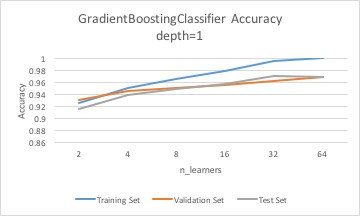
\includegraphics[width=8cm]{gradientBoost1} 
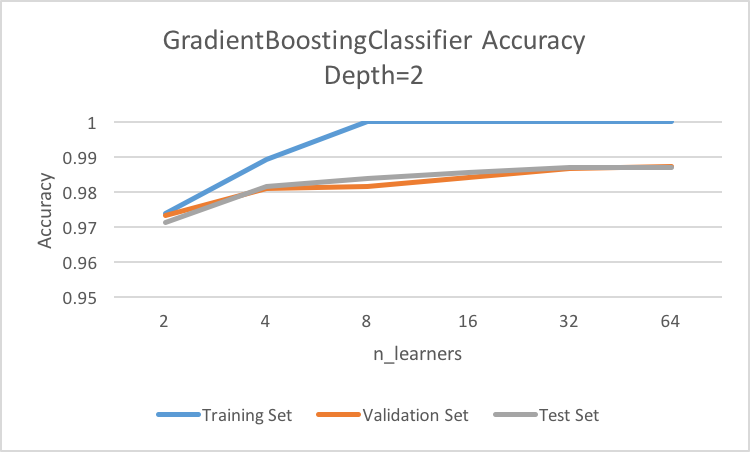
\includegraphics[width=8cm]{gradientBoost2} 
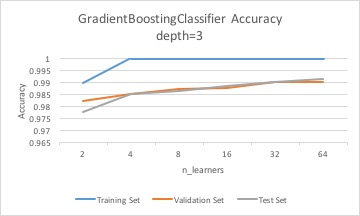
\includegraphics[width=8cm]{gradientBoost3}


\end{document}  